%---------- Inleiding ---------------------------------------------------------

\section{Introductie} % The \section*{} command stops section numbering
\label{sec:introductie}

Er wordt onderzoek gedaan omtrent de meest efficiënte marketing techniek om veel mensen te bereiken, met focus op Growth Hacking. Dit onderzoek wordt gevoerd specifiek voor Kriket, een Brusselse start-up die een krekelreep 100\% op eigen bodem produceert, promoot en verdeeld. Kriket realiseert het grootste deel van hun verkopen via retailers die ze zelf zoeken, maar er is ook een webshop\footnote{zie \href{https://kriket.be}{kriket.be}}.

Het idee voor dit onderzoek kwam uit een brainstorm-sessie met Michiel en Gauthier van Kriket in hun hipster-kantoor te WTC I Brussel. Oorspronkelijk was het idee om een referral-systeem op te starten. 

Een referral-systeem houdt in dat er bijvoorbeeld een link gegenereerd kan worden voor een klant die Kriket aan zijn vrienden wilt aanraden. Op deze manier zorgen klanten voor meer klanten. Ze worden aangespoord om deze link te delen door een beloning, voor beide partijen, zoals 10\% korting of gratis krekelrepen. Het is een systeem dat vele online bedrijven gebruiken. Maar is het de beste growth hacking techniek? Daar zal deze bachelorproef meer inzicht over geven.

Het onderzoek zal steeds specifiek voor Kriket gebeuren, zoals verschillende growth hacking technieken (theoretisch) toepassen. Ook gaat er bekeken worden of growth hacking het volledige (traditionele of digitale) marketing departement binnen een start-up kan vervangen.

Tot slot er focus gelegd worden op wélke growth hack Kriket kan gebruiken. De meeste growth hacking voorbeelden komen uit online start-ups zoals Airbnb, Dropbox, Spotify, Hotmail, ... Daarom zal er onderzoek gedaan worden of dit ook toepasbaar is op een niet-technologische Brusselse start-up met een fysiek product.

%---------- Stand van zaken ---------------------------------------------------

\section{State-of-the-art}
\label{sec:state-of-the-art}

Growth hacking is een 'hot topic', er wordt veel over gepraat, maar toch heerst er veel onduidelijkheid over wat het exact is. Verder is het een onderwerp dat vaak gekoppeld wordt met start-ups, omdat het daarbij het meest relevant is. Tot zover zijn er enkel nog toepassingen gevonden online of technologische start-ups.

Het onderzoek~\citetitle{Lee2016} van~\textcite{Lee2016} is een goede inspiratie, er zal veel naar verwezen worden omdat het een goede basis is met degelijke bronnen. Het is belangrijk te vermelden dat dit onderzoek geen kopie wordt van de bachelor thesis van~\textcite{Lee2016}. Het toepassen van growth hacking technieken op een Brusselse start-up, die geen technologiebedrijf is, zorgt (vermoedelijk) voor een volledig andere aanpak. 

In de thesis ~\citetitle{Vunk2017} bespreekt~\textcite{Vunk2017} growth hacking technieken die gebruikt worden bij start-ups in Estland. De conclusies hiervan kunnen helpen met het vinden van geografische factoren die growth hacking technieken beïnvloeden. Zo kunnen er en verschillen vast gelegd worden met de Belgische markt en kunnen er globale conclusies getrokken worden.

Tot slot is er ook onderzoek gedaan rond start-ups die een bepaalde markt verstoren en veranderen in de master thesis van~\textcite{Bergendal2017}, ~\citetitle{Bergendal2017}. Het verstoren van een bepaalde markt (disruption) en binnen een markt groeien wordt (growth) wordt mooi naast elkaar afgebeeld. “For a business today to truly succeed, it has to either grow or disrupt. If it’s lucky, it will do both” (Patel 2015). Dit zorgt voor een extra invalshoek die niet voor de hand liggend was, er zal rekening mee gehouden worden tijdens het voeren van onderzoek in functie van Kriket. 

% Voor literatuurverwijzingen zijn er twee belangrijke commando's:
% \autocite{KEY} => (Auteur, jaartal) Gebruik dit als de naam van de auteur
%   geen onderdeel is van de zin.
% \textcite{KEY} => Auteur (jaartal)  Gebruik dit als de auteursnaam wel een
%   functie heeft in de zin (bv. ``Uit onderzoek door Doll & Hill (1954) bleek
%   ...'')

%---------- Methodologie ------------------------------------------------------
\section{Methodologie}
\label{sec:methodologie}

Een growth hacker is half marketeer en half ingenieur, zoals vermeld in onderzoek van~\textcite{Lee2016}. Men moet weten wat er technisch mogelijk is en die kennis in het achterhoofd houden wanneer er over het marketinggedeelte wordt nagedacht. 

\begin{figure}[h!]
	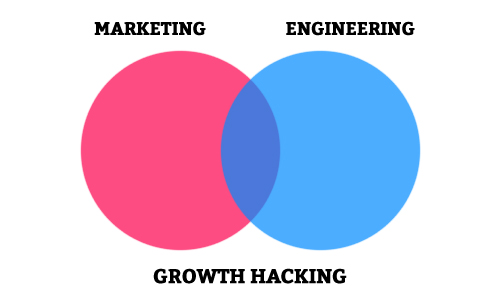
\includegraphics[width=\linewidth]{growth-hacker-definition.jpg}
	\caption{Definitie van een growth hacker, "Growth hacking as a fusion of two fields"  (Brody 2013, geciteerd 13.05.2016)}
	\label{fig:defGrowthHacker}
\end{figure}

Er zijn overigens geen vaste richtlijnen voor growth hacking, het is een opeenvolging van experimenten die gevoerd wordt om tot de ideale "hack" te komen. Men moet natuurlijk eerst brainstromen over verschillende mogelijke experimenten. Dat zal een groot deel worden vandit onderzoek zal gebeuren; experimenten bedenken en uitwerken die Kriket kunnen helpen met een versnelde groei.

Om deze experimenten te bedenken zal er eerst een klein marktonderzoek nodig zijn, eventueel door enquêtes of interviews bij andere start-ups en kleine voedselproductie bedrijven. 

Indien mogelijk zou het ook interessant zijn om een experiment uit te voeren en de groei te meten via Google en/of Facebook Analytics. Echter zullen de meeste experimenten theoretisch blijven en zal er door middel van dieper onderzoek een schatting gemaakt worden voor de slaagkansen van het experiment.

%---------- Verwachte resultaten ----------------------------------------------
\section{Verwachte resultaten}
\label{sec:verwachte_resultaten}

De behaalde resultaten zullen voornamelijk bestaan uit enkele uitgewerkte experimenten. Een experiment is in deze context dus een mogelijke "hack" die zorgt voor een versnelde community-groei specifiek voor Kriket. 

De enquêtes of interviews voor het marktonderzoek kunnen zorgen voor statistieken die in grafieken gebruikt worden.

Indien er een experiment wordt uitgevoerd kan alles gemeten worden via Analytics-tools (zoals eerder vermeld, Google en/of Facebook Analytics). Deze statistieken zullen dan veel inzichten brengen over de hoeveelheid nieuwe bezoekers en klanten, maar ook de weg die ze hebben afgelegd naar Kriket en zoveel meer.


%---------- Verwachte conclusies ----------------------------------------------
\section{Verwachte conclusies}
\label{sec:verwachte_conclusies}

Er wordt verwacht dat het vinden van growth hacking technieken voor een niet-technologische start-up minder conventioneel is dan voor technologische start-ups. Hierdoor zal er dus minder informatie over te vinden zijn en dat maakt dit natuurlijk een zinvol en uitdagend onderzoek.

Uit een uitgevoerd experiment zal hopelijk geconcludeerd kunnen worden dat er een stijging is in het aantal interesse in Kriket, hetzij via Facebook, de website of een ander kanaal.

Een groei in de Kriket-community, door dit onderzoek, zou de mooiste conclusie zijn.

